% 105-14(105쪽) — 밑면의 반지름의 길이가 10 cm, 높이가 8 cm 인 원뿔 모양의 빈 그릇에 물을 넣는 그림(수면이 올라가는 것을 화살표로 표시). 스캔 화질이 낮아 TikZ 로 다시 그림.
% 원문에 있는 것만 옮긴다: 원뿔 그릇 · 안쪽 벽 · 밑면의 반지름(10 cm)과 직각 표시 · 높이 치수 점선(8 cm) · 수면 두 자리와 올라가는 화살표. 수면 높이는 원문 그림의 비율 그대로 그려 답이 읽히지 않게 한다.
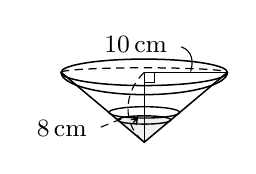
\begin{tikzpicture}[x=0.24cm, y=0.24cm, line width=0.55pt]
  % 담긴 물
  \fill[gray!12] (-1.41,1.18) arc(180:360:1.41 and 0.22) -- (0,0) -- cycle;
  \fill[gray!12] (-1.41,1.18) arc(180:0:1.41 and 0.22) -- (0,0) -- cycle;
  % 그릇
  \draw (0,3.7) ellipse (4.4 and 0.70);
  \draw (-4.4,3.7) arc(180:360:4.4 and 1.18);
  \draw[densely dashed, line width=0.45pt] (-4.4,3.7) arc(180:0:4.4 and 0.24);
  \draw (-4.4,3.7) -- (0,0) -- (4.4,3.7);
  % 높이와 밑면의 반지름
  \draw[line width=0.5pt] (0,3.7) -- (0,0);
  \draw[line width=0.5pt] (0,3.7) -- (4.4,3.7);
  \draw[line width=0.4pt] (0,3.18) -- (0.52,3.18) -- (0.52,3.7);
  % 수면
  \draw[line width=0.5pt] (0,1.58) ellipse (1.87 and 0.30);
  \draw[line width=0.5pt] (0,1.18) ellipse (1.41 and 0.22);
  \draw[->, >=stealth, line width=0.4pt] (-0.62,0.98) -- (-0.30,1.40);
  % 치수
  \draw[densely dashed, line width=0.4pt] (0,3.7) .. controls (-1.15,2.6) and (-1.15,0.9) .. (0,0);
  \draw[densely dashed, line width=0.4pt] (-2.30,0.80) -- (-1.05,1.30);
  \node[left=1.5pt, font=\small] at (-2.30,0.72) {$8\,\mathrm{cm}$};
  \draw[line width=0.4pt] (1.95,5.05) .. controls (2.55,4.85) and (2.62,4.25) .. (2.45,3.74);
  \node[left=1.5pt, font=\small] at (1.95,5.15) {$10\,\mathrm{cm}$};
\end{tikzpicture}
